% Systematic Review / Meta-analysis Manuscript Stub
% Generated by Researcher plugin: systematic-review + statistical-analysis skills (M4)
% Compile with: scripts/latex-compile.py (uses tectonic, latexmk, or pdflatex, whichever is installed)
%
% DERIVED-COUNTS CONTRACT (D10, PRISMA 2020 as a reporting VIEW over the ledger):
%   Every PRISMA count below is DERIVED from the append-only provenance ledger, never stored
%   and never hand-edited. Regenerate the \prisma... macros from the kernel:
%       uv run --project "${CLAUDE_PLUGIN_ROOT}/core" python -m researcher_core \
%           prisma flow --run-id <run> --json
%   and read the fields named in each macro comment. The values shipped here are labeled
%   PLACEHOLDERS so the stub compiles standalone; overwrite them with the derived JSON.
%   Deleting a screening event changes the derived flow, which is the property that proves
%   the numbers are derived rather than typed.
%
% NO POOLED NUMBER IS HAND-TYPED (D18). The pooled estimate, I^2, and tau^2 in the Synthesis
%   section come from the committed meta-analysis script, bound to its input-table hash and
%   environment through an experiment-run manifest. A hand edit to any of them fails
%   `researcher compile` with code C002 (altered number). See the statistical-analysis skill.

\documentclass[12pt,a4paper]{article}

\usepackage[utf8]{inputenc}
\usepackage[T1]{fontenc}
\usepackage{lmodern}
\usepackage[margin=1in]{geometry}
\usepackage{setspace}
\doublespacing

\usepackage{amsmath,amssymb}
\usepackage{graphicx}
\usepackage{booktabs}
\usepackage{array}
\usepackage{longtable}
\usepackage{multirow}
\usepackage{caption}
\usepackage{xcolor}
\usepackage{float}

\usepackage{tikz}
\usetikzlibrary{arrows.meta,positioning,shapes.geometric,calc,fit,backgrounds}

\usepackage[round,authoryear]{natbib}

\usepackage{hyperref}
\hypersetup{
    colorlinks=true,
    linkcolor=blue,
    citecolor=blue,
    urlcolor=blue
}

% --- Derived PRISMA 2020 flow counts -------------------------------------------------
% Each macro maps to ONE field of `prisma flow --json`. Regenerate; do not hand-edit.
% The placeholder values below are internally consistent so the stub renders sensibly.
\newcommand{\prismaIdentified}{412}          % flow.identified
\newcommand{\prismaIdentifiedBySource}{%
    OpenAlex 250; Crossref 120; PubMed 42}   % flow.identified_by_source (per-database)
\newcommand{\prismaDuplicates}{78}           % flow.duplicates_removed
\newcommand{\prismaAfterDedup}{334}          % flow.records_after_dedup (records screened)
\newcommand{\prismaScreened}{334}            % flow.records_screened (title/abstract decisions logged)
\newcommand{\prismaRecExcluded}{291}         % flow.records_excluded (title/abstract)
\newcommand{\prismaReportsSought}{43}        % flow.reports_sought_for_retrieval
\newcommand{\prismaReportsNotRetrieved}{5}   % flow.reports_not_retrieved
\newcommand{\prismaReportsAssessed}{38}      % flow.reports_assessed
\newcommand{\prismaReportsExcluded}{26}      % flow.reports_excluded (full-text)
\newcommand{\prismaIncluded}{12}             % flow.studies_included
% flow.reports_excluded_by_reason: one row per reason. Regenerate from the JSON dict.
\newcommand{\prismaReasonOne}{Wrong population (n = 14)}
\newcommand{\prismaReasonTwo}{No extractable outcome (n = 8)}
\newcommand{\prismaReasonThree}{Not a randomized trial (n = 4)}

% --- PRISMA flow box styles ----------------------------------------------------------
\tikzset{
    prismabox/.style={
        draw, rounded corners=1pt, align=left, font=\footnotesize\sffamily,
        text width=5.1cm, inner sep=5pt, minimum height=1.05cm, fill=blue!4},
    prismaexcl/.style={prismabox, text width=4.6cm, fill=red!4},
    prismaphase/.style={
        font=\small\sffamily\bfseries, rotate=90, anchor=center,
        text=black!70},
    prismaflow/.style={-{Latex[length=2.5mm]}, thick},
    prismaside/.style={-{Latex[length=2.5mm]}, thick},
}

\title{TITLE: A Systematic Review and Meta-analysis}
\author{
    First Author\textsuperscript{1,*} \and
    Second Author\textsuperscript{2}
    \\[1em]
    \small\textsuperscript{1}Department, University, City, Country \\
    \small\textsuperscript{2}Department, Institution, City, Country \\
    \small\textsuperscript{*}Corresponding author: \href{mailto:email@example.com}{email@example.com}
}
\date{}

\begin{document}

\maketitle

\begin{abstract}
% Background, Objectives, Data sources, Study eligibility criteria, Methods,
% Results (with the derived counts), Limitations, Conclusions, Registration.
% PRISMA 2020 abstract checklist items are author-supplied prose.
\end{abstract}

\tableofcontents
\newpage

\section{Introduction}
% Rationale (PRISMA 2020 item 3) and Objectives (item 4). Author-supplied prose.
% State the review question in the framing used to lock the protocol (PICO, PECO, or SPIDER).

\section{Methods}

\subsection{Protocol and registration}
% PRISMA 2020 items 24a and 24b. The protocol was locked before screening began; its content
% hash and every amendment live in the ledger (protocol_locked and amendment events). List all
% amendments here with what changed, why, and when. If the protocol was unchanged, state
% ``no amendments''. Do not describe a deviation as an edit: the ledger shows the locked original.

\subsection{Eligibility criteria}
% PRISMA 2020 item 5. Transcribe the locked eligibility profile (PICO/PECO/SPIDER elements with
% per-element include/exclude criteria). These are the same qualifier axes the evidence edges carry.

\subsection{Information sources and search strategy}
% PRISMA 2020 items 6 and 7. Every source and its VERBATIM query string are recorded as retrieval
% events. Reproduce the exact per-database strategy in the appendix (Table~\ref{tab:strategies}),
% byte-for-byte from the ledger, not a paraphrase.

\subsection{Selection process}
% PRISMA 2020 item 8. Two independent screeners per record; conflicts resolved by BLINDED
% adjudication (the adjudicator saw the record and the profile, not the two votes). Cohen's kappa
% between streams was derived from the ledger and is reported below. If single-screener mode was
% used, say so here as a stated limitation.

\subsection{Data collection and risk-of-bias assessment}
% PRISMA 2020 items 9, 10, 11. Extraction used typed columns anchored to full-text passages where
% available and abstract otherwise; abstract-only cells are labeled and never presented as
% full-text-verified. Risk of bias used RoB 2 for randomized trials; certainty of evidence used
% GRADE. No automated risk-of-bias scoring was applied; every judgment was made by a human, and
% each completed worksheet is hashed into the ledger.

\subsection{Synthesis and certainty}
% PRISMA 2020 items 13a-13f. Name the effect measure, the model (fixed vs random effects), the
% heterogeneity estimator, and the small-study-effects assessment. All synthesis numbers are
% generated by the committed meta-analysis script (Section~\ref{sec:synthesis}); none is hand-typed.

\section{Results}

\subsection{Study selection}
\label{sec:selection}
% PRISMA 2020 item 16a. The flow below is DERIVED from the ledger (`prisma flow`); the macros in
% the preamble hold the JSON fields. Both views (figure and table) read the SAME macros, so they
% cannot disagree.

\begin{figure}[htbp]
\centering
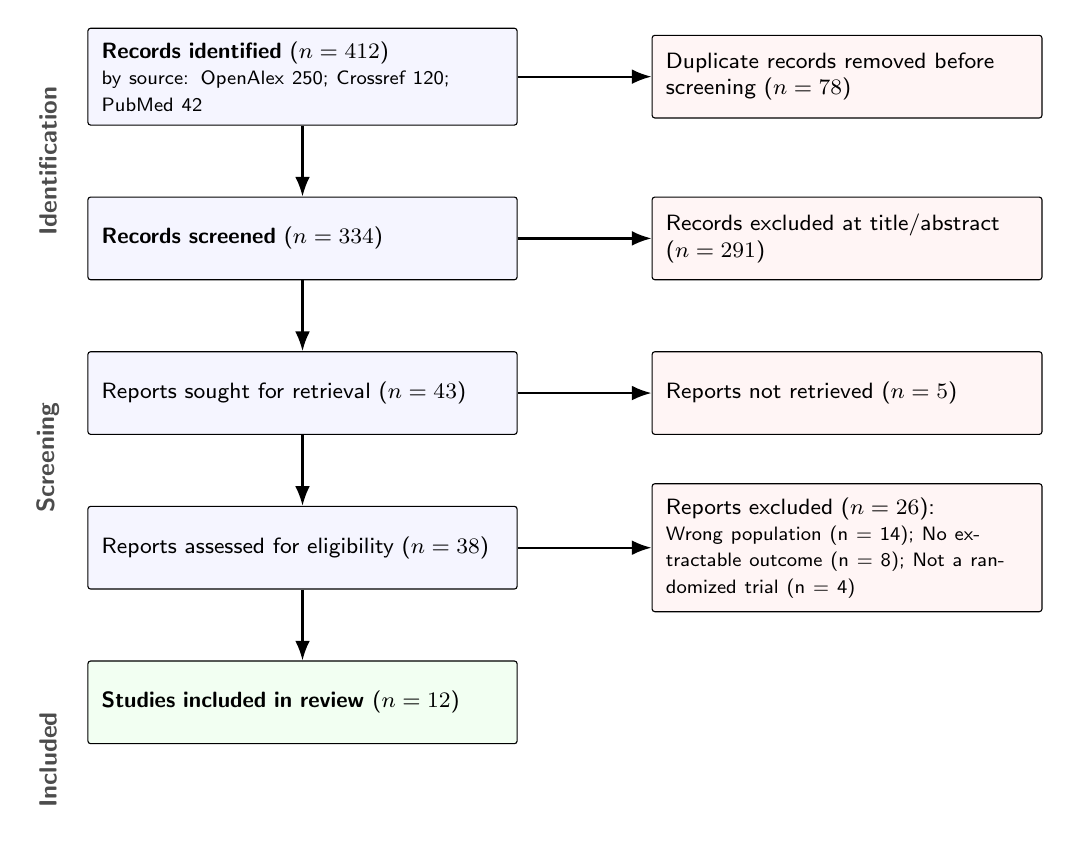
\begin{tikzpicture}[node distance=0.9cm and 1.7cm]

    % --- Identification -----------------------------------------------------------
    \node[prismabox] (id) {%
        \textbf{Records identified} ($n = \prismaIdentified$)\\
        {\scriptsize by source: \prismaIdentifiedBySource}};
    \node[prismaexcl, right=of id] (rem) {%
        Duplicate records removed before screening ($n = \prismaDuplicates$)};

    % --- Screening: title/abstract ------------------------------------------------
    \node[prismabox, below=of id] (scr) {%
        \textbf{Records screened} ($n = \prismaAfterDedup$)};
    \node[prismaexcl, right=of scr] (exc1) {%
        Records excluded at title/abstract ($n = \prismaRecExcluded$)};

    % --- Screening: retrieval -----------------------------------------------------
    \node[prismabox, below=of scr] (sought) {%
        Reports sought for retrieval ($n = \prismaReportsSought$)};
    \node[prismaexcl, right=of sought] (notret) {%
        Reports not retrieved ($n = \prismaReportsNotRetrieved$)};

    % --- Screening: eligibility ---------------------------------------------------
    \node[prismabox, below=of sought] (assess) {%
        Reports assessed for eligibility ($n = \prismaReportsAssessed$)};
    \node[prismaexcl, right=of assess] (exc2) {%
        Reports excluded ($n = \prismaReportsExcluded$):\\
        {\scriptsize \prismaReasonOne; \prismaReasonTwo; \prismaReasonThree}};

    % --- Included -----------------------------------------------------------------
    \node[prismabox, below=of assess, fill=green!5] (inc) {%
        \textbf{Studies included in review} ($n = \prismaIncluded$)};

    % --- Flow arrows --------------------------------------------------------------
    \draw[prismaflow] (id) -- (scr);
    \draw[prismaflow] (scr) -- (sought);
    \draw[prismaflow] (sought) -- (assess);
    \draw[prismaflow] (assess) -- (inc);
    \draw[prismaside] (id) -- (rem);
    \draw[prismaside] (scr) -- (exc1);
    \draw[prismaside] (sought) -- (notret);
    \draw[prismaside] (assess) -- (exc2);

    % --- Phase labels -------------------------------------------------------------
    \node[prismaphase, left=0.5cm of id] {Identification};
    \node[prismaphase, left=0.5cm of sought] {Screening};
    \node[prismaphase, left=0.5cm of inc] {Included};

\end{tikzpicture}
\caption{PRISMA 2020 flow of study selection. Every count is DERIVED from the provenance ledger
via \texttt{researcher-core prisma flow}; the values shown are labeled placeholders in the
template and are overwritten from the derived JSON. This figure and Table~\ref{tab:prisma-flow}
read the same source macros.}
\label{fig:prisma}
\end{figure}

% Plain-table mirror of the same derived counts (accessibility and copy-paste into text).
\begin{table}[htbp]
\centering
\caption{PRISMA 2020 flow counts, derived from the ledger (\texttt{prisma flow}).}
\label{tab:prisma-flow}
\begin{tabular}{@{}l r@{}}
\toprule
\textbf{PRISMA 2020 stage} & \textbf{$n$ (derived)} \\
\midrule
Records identified (all databases)        & \prismaIdentified \\
\quad by source: \prismaIdentifiedBySource & \\
Duplicate records removed                 & \prismaDuplicates \\
Records screened (after deduplication)    & \prismaAfterDedup \\
\quad title/abstract decisions logged     & \prismaScreened \\
Records excluded at title/abstract        & \prismaRecExcluded \\
Reports sought for retrieval              & \prismaReportsSought \\
Reports not retrieved                     & \prismaReportsNotRetrieved \\
Reports assessed for eligibility          & \prismaReportsAssessed \\
Reports excluded (with reasons)           & \prismaReportsExcluded \\
\quad \prismaReasonOne                     & \\
\quad \prismaReasonTwo                     & \\
\quad \prismaReasonThree                   & \\
\textbf{Studies included in review}       & \textbf{\prismaIncluded} \\
\bottomrule
\end{tabular}
\end{table}

\subsection{Screening agreement}
% Report Cohen's kappa between the two screening streams (derived: `screen kappa`) and the number
% of conflicts resolved by blinded adjudication. State the interpretation band used.

\subsection{Study characteristics and risk of bias}
% PRISMA 2020 items 17 and 18. One row per included study from the extraction table; the RoB 2
% domain judgments render into Table~\ref{tab:rob2}. Cells anchored only at abstract level are
% labeled; genuinely absent data reads ``not reported'', never a fabricated value.

\begin{table}[htbp]
\centering
\caption{Risk of bias (RoB 2) across the included randomized trials. Domain judgments are
human-completed worksheet outputs hashed into the ledger; this table cites those worksheet hashes.}
\label{tab:rob2}
\begin{tabular}{@{}l c c c c c c@{}}
\toprule
\textbf{Study} & \textbf{D1} & \textbf{D2} & \textbf{D3} & \textbf{D4} & \textbf{D5} & \textbf{Overall} \\
\midrule
Study A (2021) & Low  & Low  & Some & Low  & Low  & Some concerns \\
Study B (2022) & Low  & Low  & Low  & Low  & Low  & Low \\
% ... one row per included study; D1-D5 are the RoB 2 domains.
\bottomrule
\end{tabular}
\end{table}

\subsection{Synthesis of results}
\label{sec:synthesis}
% PRISMA 2020 items 20a-20d. THE NUMBERS BELOW ARE SCRIPT-GENERATED, NOT TYPED. The forest plot,
% the pooled estimate, its confidence interval, I^2, and tau^2 all come from the committed
% meta-analysis script (see the statistical-analysis skill, Meta-analysis section). Each is an
% INTERNAL evidence edge in the lineage graph, bound to the script's experiment-run manifest
% (code commit, input extraction-table hash, environment lockfile hash, artifact hashes) per D18.
% A hand edit to any pooled number changes the artifact content without updating the manifest,
% so `researcher compile` reports C002 (altered number) and the gate fails. Do not retype them.

\begin{figure}[htbp]
\centering
% Replace this placeholder with the generated figure once the script has run:
%   \includegraphics[width=0.9\textwidth]{figures/forest.pdf}
\fbox{\parbox[c][4.5cm][c]{0.9\textwidth}{\centering\sffamily
    \textbf{Forest plot placeholder}\\[4pt]
    Generated by the committed meta-analysis script.\\
    Pooled estimate, confidence interval, and weights are read from
    \texttt{figures/pooled-estimates.json}; never typed here.}}
\caption{Forest plot of the pooled effect. Generated by \texttt{scripts/meta\_analysis.py} from
the committed extraction table; the pooled estimate is a compile-bound internal evidence edge.}
\label{fig:forest}
\end{figure}

% GRADE summary-of-findings scaffold. Certainty ratings are human GRADE judgments; the pooled
% effect column is filled from the derived JSON, never typed.
\begin{table}[htbp]
\centering
\caption{GRADE summary of findings. Certainty is the human worksheet judgment (cited by hash);
the effect column is the script-generated pooled estimate.}
\label{tab:grade}
\begin{tabular}{@{}l c c c@{}}
\toprule
\textbf{Outcome} & \textbf{Studies ($n$)} & \textbf{Pooled effect (95\% CI)} & \textbf{Certainty} \\
\midrule
Primary outcome   & \prismaIncluded & \textit{[from pooled-estimates.json]} & Moderate \\
% ... one row per outcome; effect cells are script-generated, certainty is GRADE.
\bottomrule
\end{tabular}
\end{table}

\subsection{Heterogeneity and reporting biases}
% PRISMA 2020 items 20c and 21. Report I^2 (with its CI), tau^2, and the prediction interval,
% all from the script. Report the funnel plot and small-study-effects test (for example Egger's,
% when at least 10 studies) and feed asymmetry into the GRADE publication-bias domain.

\section{Discussion}
% PRISMA 2020 items 23a-23d. Interpretation, limitations of the evidence (item 23a is
% author-supplied), limitations of the review process, and implications.

\section{Conclusion}
% Key findings and their certainty, in the words the GRADE table supports.

\section*{Acknowledgments}

\appendix

\section{Search strategies (verbatim)}
\label{app:strategies}
% PRISMA 2020 item 7. Each row is the EXACT query string from a retrieval event, reproduced
% byte-for-byte from the ledger. Do not paraphrase.
\begin{table}[htbp]
\centering
\caption{Per-database search strategies, reproduced verbatim from the ledger retrieval events.}
\label{tab:strategies}
\begin{tabular}{@{}l l r@{}}
\toprule
\textbf{Source} & \textbf{Verbatim query} & \textbf{Identified} \\
\midrule
OpenAlex & \texttt{[exact filter expression]} & 250 \\
Crossref & \texttt{[exact query]}              & 120 \\
PubMed   & \texttt{[exact term string with field tags]} & 42 \\
% ... one row per source in the protocol.
\bottomrule
\end{tabular}
\end{table}

\section{PRISMA 2020 checklist coverage}
\label{app:checklist}
% DERIVED from the ledger via `prisma checklist`. Each item is either satisfied by ledger
% evidence (``derived''), not yet satisfied (``missing''), or ``author-supplied'' when no event
% can stand in for the author's prose. Regenerate this table from the JSON; do not hand-edit the
% status column.
\begin{longtable}{@{}l l l l@{}}
\caption{PRISMA 2020 checklist coverage, derived from the ledger (\texttt{prisma checklist}).}
\label{tab:checklist} \\
\toprule
\textbf{Item} & \textbf{Section} & \textbf{Name} & \textbf{Status} \\
\midrule
\endfirsthead
\toprule
\textbf{Item} & \textbf{Section} & \textbf{Name} & \textbf{Status} \\
\midrule
\endhead
\bottomrule
\endfoot
3   & Introduction      & Rationale                    & author-supplied \\
4   & Introduction      & Objectives                   & author-supplied \\
5   & Methods           & Eligibility criteria         & derived \\
6   & Methods           & Information sources          & derived \\
7   & Methods           & Search strategy              & derived \\
8   & Methods           & Selection process            & derived \\
9   & Methods           & Data collection process      & author-supplied \\
16a & Results           & Study selection (flow)       & derived \\
16b & Results           & Studies excluded with reasons & derived \\
23a & Discussion        & Limitations of the evidence  & author-supplied \\
24a & Other information & Registration and protocol    & derived \\
24b & Other information & Amendments to the protocol   & author-supplied \\
\end{longtable}

\bibliographystyle{plainnat}
\bibliography{references/library}

\end{document}
